\documentclass[border=4pt]{standalone}
\usepackage{amsmath,amssymb,tikz}
\usetikzlibrary{arrows.meta,calc,matrix,positioning}
\definecolor{figB}{RGB}{31,90,166}\definecolor{figR}{RGB}{176,48,48}\definecolor{figG}{RGB}{46,125,50}\definecolor{figO}{RGB}{214,120,20}
\begin{document}
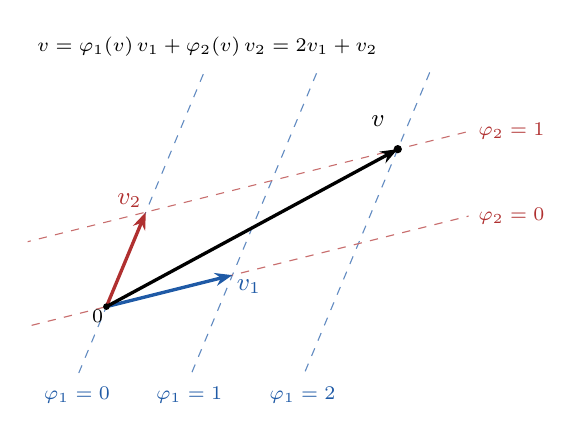
\begin{tikzpicture}[scale=1.0,>={Stealth[length=2.2mm]}]
% basis v1=(1.6,0.4), v2=(0.5,1.2); v = 2v1 + v2 = (3.7,2.0)
\begin{scope}
\clip (-1.0,-0.9) rectangle (4.6,3.0);
\foreach \c in {0,1,2} \draw[figB!70,thin,dashed] ({\c*1.6-2*0.5},{\c*0.4-2*1.2})--({\c*1.6+3*0.5},{\c*0.4+3*1.2});
\foreach \c in {0,1} \draw[figR!70,thin,dashed] ({-2*1.6+\c*0.5},{-2*0.4+\c*1.2})--({4*1.6+\c*0.5},{4*0.4+\c*1.2});
\end{scope}
\node[font=\scriptsize,figB,anchor=north] at ({0*1.6-0.75*0.5},-0.9) {$\varphi_1=0$};
\node[font=\scriptsize,figB,anchor=north] at ({1*1.6-0.4*0.5-0.35},-0.9) {$\varphi_1=1$};
\node[font=\scriptsize,figB,anchor=north] at ({2.49},-0.9) {$\varphi_1=2$};
\node[font=\scriptsize,figR,anchor=west] at (4.6,{(4.6)*0.25}) {$\varphi_2=0$};
\node[font=\scriptsize,figR,anchor=west] at (4.6,{(4.6-0.5)*0.25+1.2}) {$\varphi_2=1$};
\draw[->,very thick,figB] (0,0)--(1.6,0.4) node[below right,font=\small,inner sep=1pt]{$v_1$};
\draw[->,very thick,figR] (0,0)--(0.5,1.2) node[above left,font=\small,inner sep=1pt]{$v_2$};
\draw[->,very thick] (0,0)--(3.7,2.0);
\node[font=\small] at (3.45,2.35) {$v$};
\fill (3.7,2.0) circle (1.5pt);
\fill (0,0) circle (1.2pt) node[below left,font=\scriptsize,inner sep=1pt]{$0$};
\node[font=\scriptsize,anchor=north west,align=left] at (-1.0,3.55) {$v=\varphi_1(v)\,v_1+\varphi_2(v)\,v_2=2v_1+v_2$};
\end{tikzpicture}
\end{document}
